\documentclass{beamer}
\mode<presentation>
\usetheme{CambridgeUS}
\usepackage[russian]{babel}
\usepackage[utf8]{inputenc}
\usepackage[T2A]{fontenc}
\usepackage{sansmathaccent}

\usepackage{verbatim}
\usepackage{alltt}

\pdfmapfile{+sansmathaccent.map}
\title[UX Elements]{Дизайн интерфейса, навигации и информационный дизайн}
\author{Наумов Д.А., доц. каф. КТ}
\date[07.10.2020] {Компьютерная графика и проектирование графических интерфейсов, 2020}

\begin{document}

%ТИТУЛЬНЫЙ СЛАЙД
\begin{frame}
  \titlepage
\end{frame}
  
%СОДЕРЖАНИЕ ЛЕКЦИИ
\begin{frame}
  \frametitle{Содержание лекции}
  \tableofcontents  
\end{frame}

\section{Уровень компоновки}
  
\begin{frame}[t]
\begin{block}{Уровень конмпоновки}
определяет, какую форму примет функциональность, определенная на уровне структуры.
\end{block}
\begin{figure}[h]
\centering
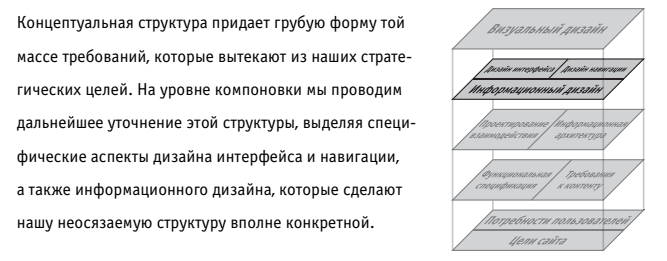
\includegraphics[scale=0.6]{images/lec04-pic01.png}
\end{figure}
Рассматриваются отдельные страницы и их составне части.
\end{frame} 

\begin{frame}[t]
\begin{figure}[h]
\centering
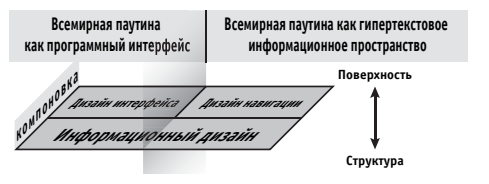
\includegraphics[scale=0.6]{images/lec04-pic02.png}
\end{figure}
\begin{itemize}
\item  дизайном интерфейса - \textbf{возможность совершать действия} - управление кнопками, полями ввода и прочими элементами интерфейса; 
\item  дизайн навигации – \textbf{возможность перейти на другую страницу} - представлением информационных пространств;
\item  информационный дизайн - \textbf{донесение идеи до пользователя} - максимально доходчивое представление информации.
\end{itemize}
\end{frame} 

\subsection{Дизайн интерфейса}

\begin{frame}[t]{Соглашение и метафора}
\begin{figure}[h]
\centering
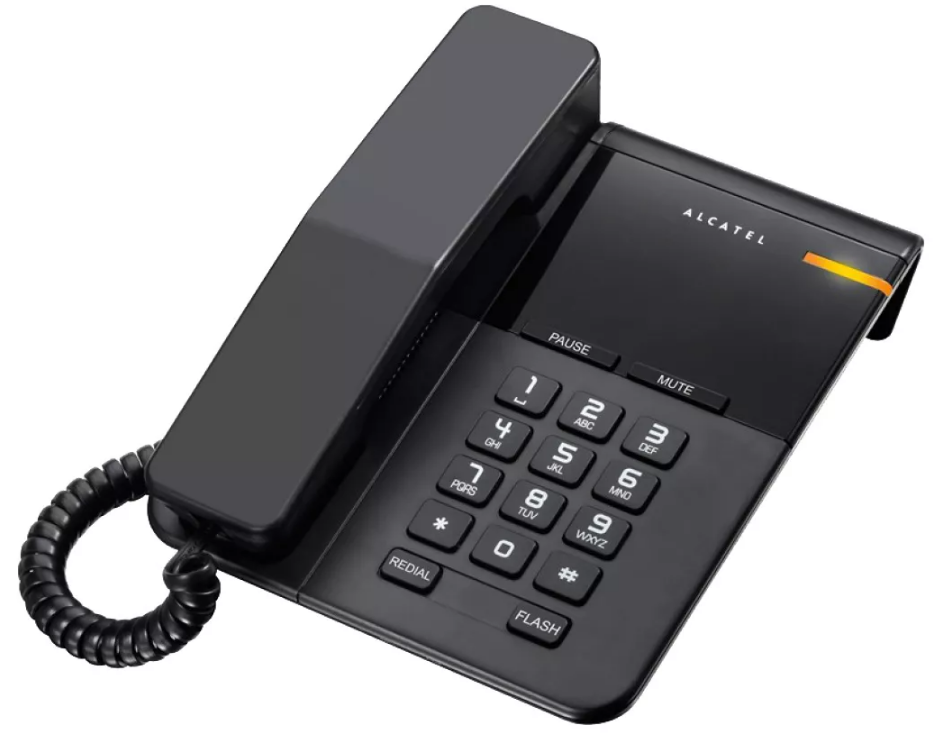
\includegraphics[scale=0.25]{images/lec04-pic03.png}
\end{figure}
\begin{itemize}
\item следование общепринятым соглашениям и метафорам;
\item создание внутренне согласованного интерфейса.
\end{itemize}
Пример: кнопка <<сохранить>>, информационные сообщения.
\end{frame} 

\begin{frame}[t]{Дизайн интерфеса}
\begin{block}{Цель дизайна интерфеса}
определить, какие аспекты не нужны пользователям, и перевести их в разряд неприметных (или исключить вообще).
\end{block}
\begin{itemize}
\item учесть наиболее вероятные линии поведения пользователей;
\item продумать опции по-умолчанию.
\item автоматически запоминать опции при последнем визите.
\end{itemize}
\begin{figure}[h]
\centering
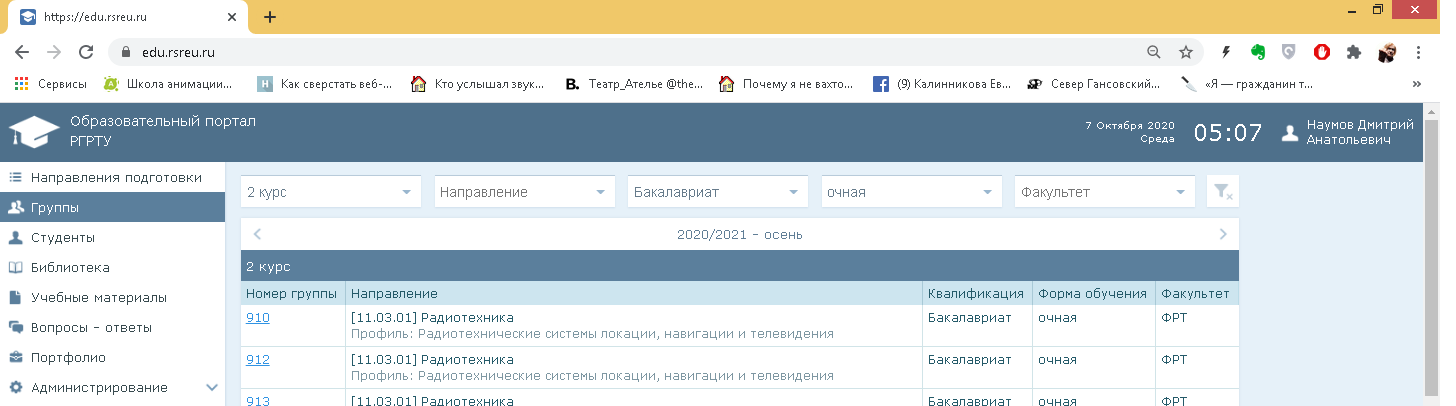
\includegraphics[scale=0.25]{images/lec04-pic04.png}
\end{figure}
\end{frame} 

\begin{frame}[t]{Ограничение технологий: HTML}
Флажки позволяют пользователям выбирать опции, не зависящие друг от друга.
\begin{figure}[h]
\centering

\includegraphics[scale=0.5]{images/lec04-pic05.png}
\end{figure}

Кнопки переключатели позволяют пользователю выбрать одну из взаимоисключающих опций.
\begin{figure}[h]
\centering

\includegraphics[scale=0.5]{images/lec04-pic06.png}
\end{figure}

Кнопки могут выполнять самые разные действия. 
\begin{figure}[h]
\centering

\includegraphics[scale=0.5]{images/lec04-pic10.png}
\end{figure}
\end{frame}

\begin{frame}[t]
Текстовые поля позволяют пользователям вводить текст.
\begin{figure}[h]
\centering

\includegraphics[scale=0.5]{images/lec04-pic07.png}
\end{figure}

Раскрывающиеся списки обеспечивают ту же функциональность, что и переключатели, но занимают меньше экранного места, позволяя использовать его более эффективно.
\begin{figure}[h]
\centering
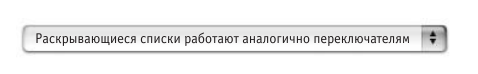
\includegraphics[scale=0.5]{images/lec04-pic08.png}
\end{figure}

Списки обеспечивают ту же функциональность, что и флажки, но занимают меньше места на экране, потому что предоставляют возможность прокрутки содержимого. 
\begin{figure}[h]
\centering
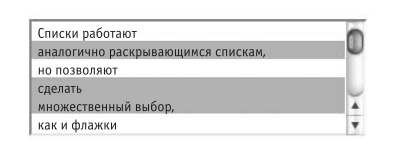
\includegraphics[scale=0.5]{images/lec04-pic09.png}
\end{figure}
\end{frame}

\begin{frame}[t]
\begin{figure}[h]
\centering
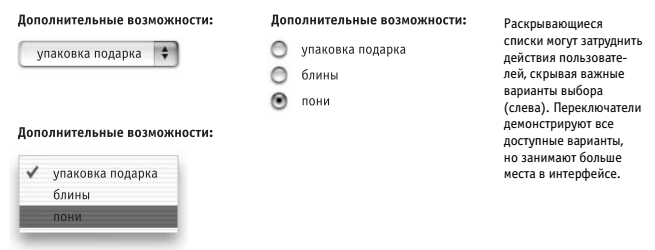
\includegraphics[scale=0.5]{images/lec04-pic11.png}
\end{figure}
Стандрантые задачи информационного дизайна:
\begin{itemize}
\item выдача сообщений об ошибках;
\item предоставление инструкций пользователю.
\end{itemize}
\end{frame}

\subsection{Дизайн навигации}
\begin{frame}[t]{Дизайн навигации}
Дизайн навигации: необходимо расставить на каждой странице ссылки, чтобы пользователь смог ориентироваться на сайте. 

Задачи:
\begin{itemize}
\item должен предоставлять пользователям способ попасть из одной точки сайта в другую; 
	\begin{itemize}
	\item невозможно связать каждую страницу с каждой;
	\item необходимо упростить перемещения пользователя;	
	\end{itemize}
\item должен отражать взаимоотношения между внутренними элементами навигации;
	\begin{itemize}
	\item как ссылки относятся друг с другом?
	\item являются ли одни ссылки более важными?
	\item пользователи должны понимать, какой у них выбор.
	\end{itemize}
\item должен отражать связь между содержательной стороной элементов навигации и страницей, которая находится перед глазами пользователя.
	\begin{itemize}
	\item какое отношение к страницам имеет этот набор ссылок?
	\item как пользователю лучше достичь цели?
	\end{itemize}	
\end{itemize}
\end{frame}

\begin{frame}[t]{Глобальная навигация}
Глобальная навигация представляет собой набор точек входа, которые необходимы пользователям, чтобы переходить с одного <<конца>> сайта на другой.
\begin{figure}[h]
\centering
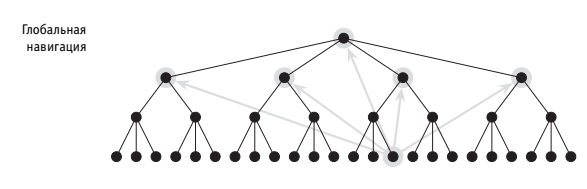
\includegraphics[scale=0.5]{images/lec04-pic12.png}
\end{figure}

Глобальная навигация не обязательно появляется на каждой странице сайта.
\end{frame}

\begin{frame}[t]{Локальная навигация}
Локальная навигация предоставляет пользователям доступ к <<ближайшим>> элементам архитектуры. 

В строго иерархической архитектуре локальная навигация может,
например, обеспечить доступ к родительской странице, страницам-потомкам и страницам-соседям. 
\begin{figure}[h]
\centering
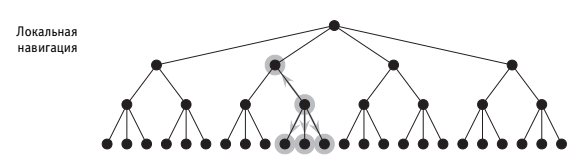
\includegraphics[scale=0.5]{images/lec04-pic13.png}
\end{figure}
Локальная навигация, как правило, оказывается наиболее часто востребованной, нежели другие варианты навигации.
\end{frame}

\begin{frame}[t]{Дополнительная навигация}
\textbf{Дополнительная навигация} обеспечивает более быстрый доступ к связанному с текущей страницей контенту, который может не быть напрямую доступным посредством глобальной или локальной навигации.
\begin{figure}[h]
\centering
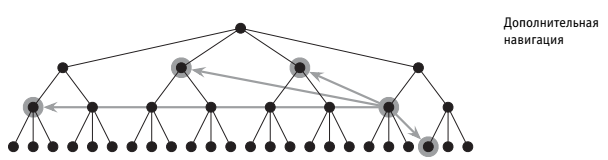
\includegraphics[scale=0.5]{images/lec04-pic14.png}
\end{figure}
\begin{itemize}
\item дает пользователям возможность переместить фокус своих изысканий на другие элементы контента без необходимости возврата в стартовую точку;
\item сохранить преимущественно иерархическую архитектуру сайта.
\end{itemize}
\end{frame}

\begin{frame}[t]{Контекстная навигация}
\textbf{Контекстная навигация} встроена непосредственно в содержимое страницы (и поэтому иногда называется микронавигацией). 
\begin{figure}[h]
\centering
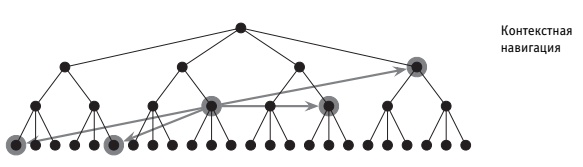
\includegraphics[scale=0.5]{images/lec04-pic15.png}
\end{figure}
Почему бы не поместить соответствующую ссылку прямо в тексте, не заставляя пользователя просматривать страницу вдоль и поперек в поисках необходимого навигацион ного элемента?
\end{frame}

\begin{frame}[t]{Сервисная навигация}
\textbf{Сервисная навигация} предоставляет доступ к элементам, которые не нужны пользователю повседневно, но которые принято предоставлять ради его удобства:
\begin{itemize}
\item cсылки на контактную информацию; 
\item cсылки на формы обратной связи; 
\item формулировка политики сайта являются распространенными элементами сервисной навигации.
\end{itemize} 
\begin{figure}[h]
\centering
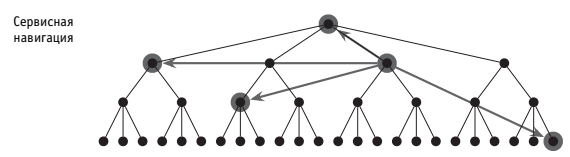
\includegraphics[scale=0.5]{images/lec04-pic16.png}
\end{figure}
\end{frame}

\begin{frame}[t]{Выносная навигация}
К \textbf{выносной навигации} пользователи обращаются тогда, когда запутались в предоставленных прочих навигационных системах или пришли к выводу, что не стоит и пытаться в них разобраться.
\begin{itemize}
\item \textbf{карта сайта} - имеет вид иерархического списка, состоящего из ссылок на разделы верхнего уровня, под которыми с отступом размещены ссылки на разделы второго уровня; 
\end{itemize} 
\begin{figure}[h]
\centering
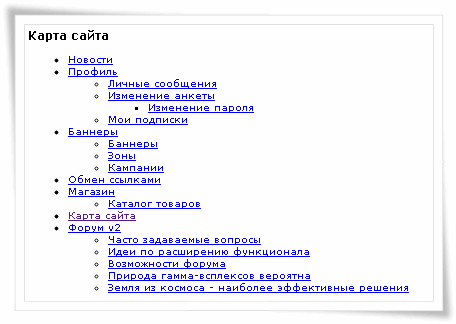
\includegraphics[scale=0.5]{images/lec04-pic17.png}
\end{figure}
\end{frame}

\begin{frame}[t]{Выносная навигация}
\begin{itemize}
\item \textbf{индекс} - алфавитный список тем со ссылками на соответствующие страницы, аналогичный предметному указателю в конце книги.
\end{itemize} 
\begin{figure}[h]
\centering
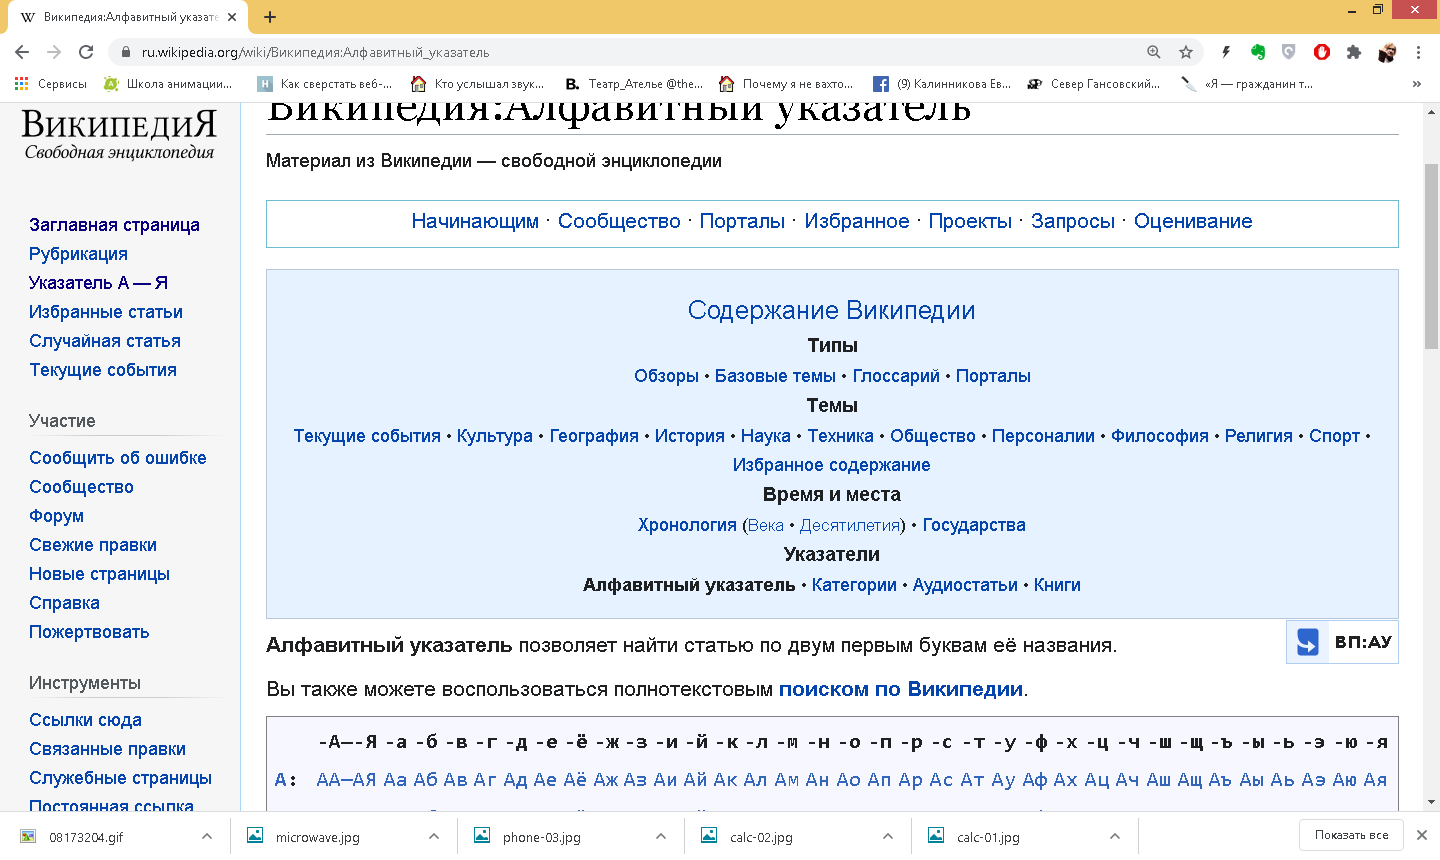
\includegraphics[scale=0.25]{images/lec04-pic18.png}
\end{figure}
\end{frame}

\subsection{Информационный дизайн}
\begin{frame}[t]{Информационный дизайн}
\begin{block}{Информационный дизайн}
сводится к принятию решений о том, как представить информацию, чтобы людям было легче воспринимать и использовать ее.
\end{block}
\begin{itemize}
\item Будет ли секторная диаграмма оптимальной для представления этих данных или нашим пользователям лучше подойдет гистограмма?
\item Сможет ли пиктограмма с биноклем адекватно передать понятие «поиск на сайте»
или пиктограмма увеличительного стекла будет понятнее?
\end{itemize} 
\end{frame}

\begin{frame}[t]{Информационный дизайн}
\begin{figure}[h]
\centering
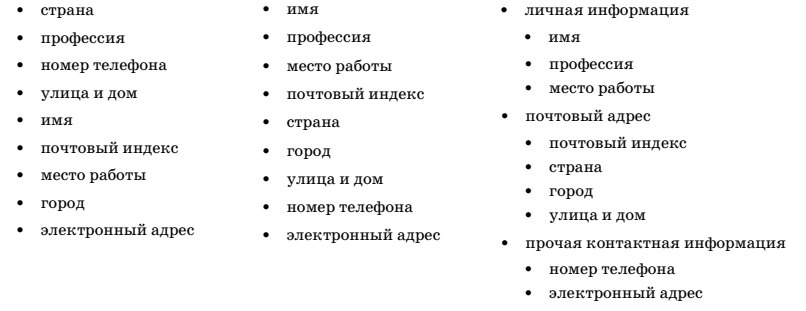
\includegraphics[scale=0.6]{images/lec04-pic19.png}
\end{figure}
\end{frame}

\begin{frame}[t]{Информационный дизайн}
Задача: сгруппировать и организовать элементы информации специальным образом, который отражает способ мышления ваших пользователей и помогает им в решении их задач и достижении их целей.
\begin{figure}[h]
\centering

\includegraphics[scale=0.6]{images/lec04-pic20.png}
\end{figure}
\end{frame}

\begin{frame}[t]{Прототипы страниц}
\textbf{Макет страницы }должен включать в себя:
\begin{itemize}
\item все навигационные системы, имеющиеся на сайте и отражающие разные взгляды на архитектуру сайта; 
\item все элементы интерфейса, необходимые для использования функциональности этой страницы; 
\item информационный дизайн, поддерживающий как вышеупомянутые элементы, 
\item контент страницы.
\end{itemize}
\end{frame}

\begin{frame}[t]{Прототипы страниц}
\textbf{Прототип страниц }- схематическое представление всех компонентов страницы и их взаимного
расположения.
\begin{figure}[h]
\centering
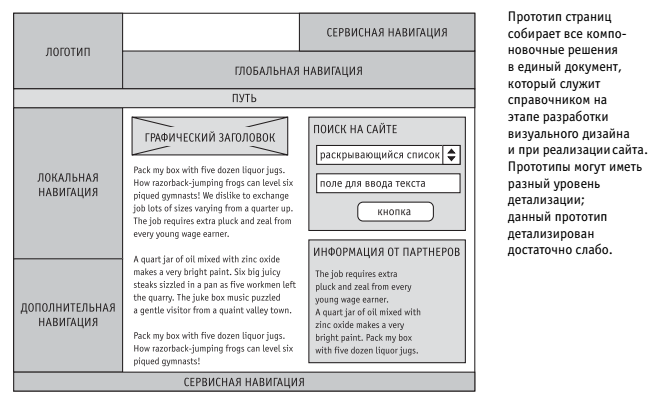
\includegraphics[scale=0.6]{images/lec04-pic21.png}
\end{figure}
\end{frame}

\begin{frame}[t]{Прототипы страниц}
\textbf{Значимость прототипов}: объединяют все три элемента уровня структуры -
\begin{itemize}
\item дизайн интерфейса – через расположение и выбор элементов
интерфейса; 
\item дизайн навигации – через идентификацию и задание главных навигационных систем;
\item информационный дизайн – через размещение и расстановку по приоритету информационных компонентов. 
\end{itemize}
Собрав эти три составляющие в одном документе, прототип способен задать компоновку, в полной мере опирающуюся на концептуальную структуру сайта и указывающую дорогу к визуальному дизайну.
\end{frame}

%\section{Уровень компоновки}

\begin{frame}[t]{ПО для создания прототипов интерфейсов}
\begin{itemize}
\item Axure RP
\item Balsamic
\end{itemize}
\begin{figure}[h]
\centering
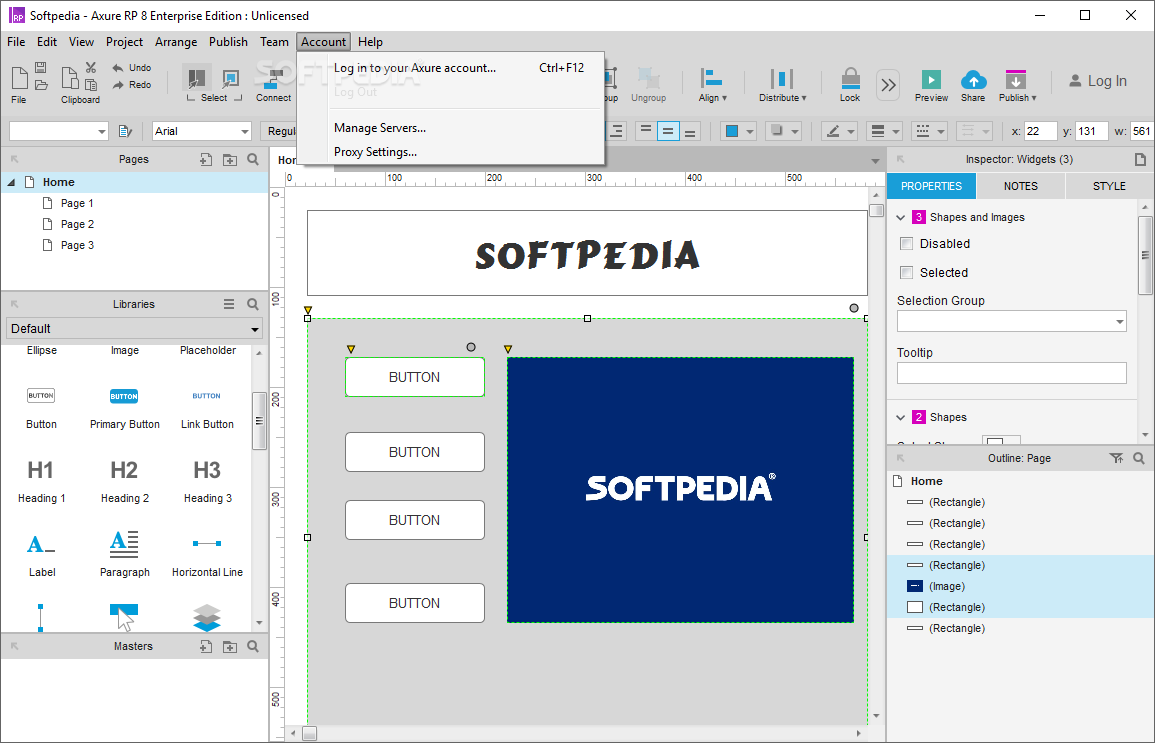
\includegraphics[scale=0.25]{images/axure-1.png}
\end{figure}
\end{frame}

\begin{frame}[t]{ПО для создания прототипов интерфейсов}
\begin{itemize}
\item Axure RP
\item Balsamic
\end{itemize}
\begin{figure}[h]
\centering
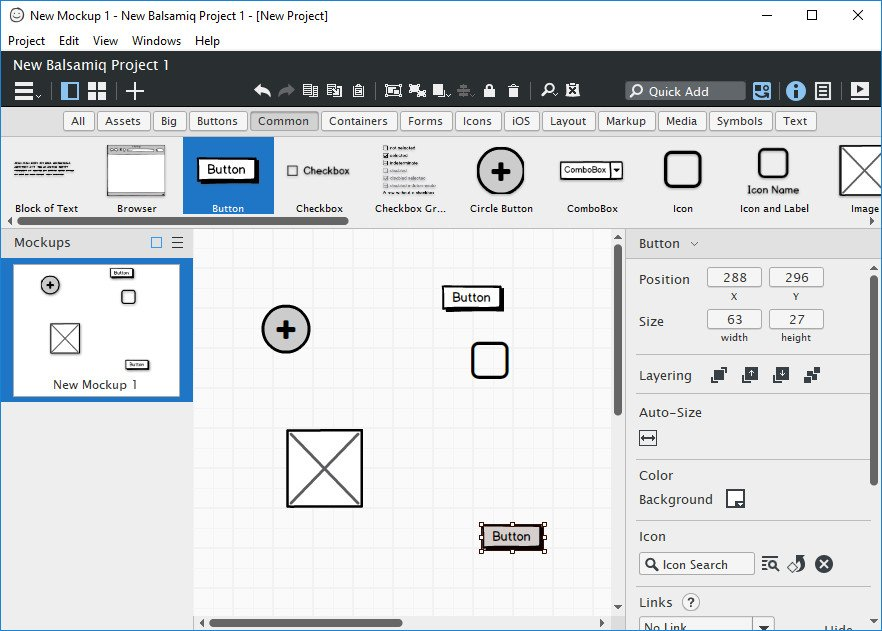
\includegraphics[scale=0.25]{images/balsamiq.jpg}
\end{figure}
\end{frame}

\begin{frame}[t]{ПО для создания прототипов интерфейсов}
\begin{itemize}
\item Axure RP
\item Balsamic
\end{itemize}
\begin{figure}[h]
\centering
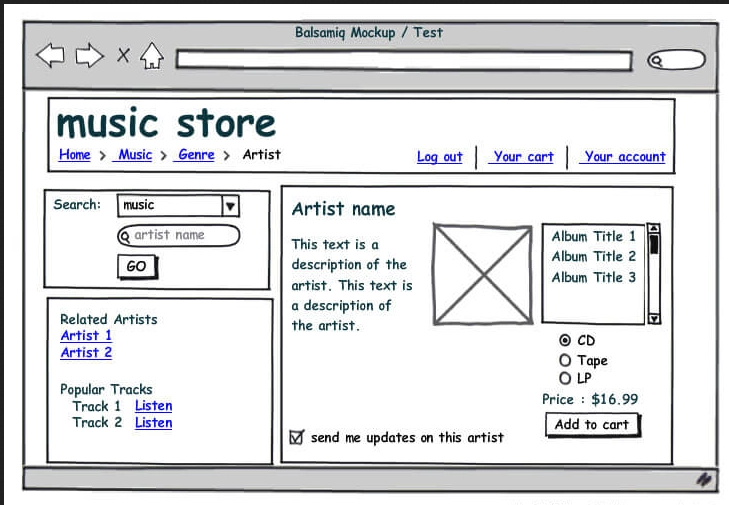
\includegraphics[scale=0.4]{images/balsamiq-1.png}
\end{figure}
\end{frame}

\begin{frame}[t]{Этапы создания прототипов}
\begin{enumerate}
\item Самое сложное – спроектировать первый макет. 
\item На первом макете будет спроектирован общий каркас: шапка, главное меню, подвал и т.д. 
\item Важно продумать, что именно пользователю может понадобиться на этой странице, и заложить все нужные блоки и ссылки. 
\item Самые важные функции мы можем изобразить в виде блоков с развернутой информацией в контентной части, туда мы помещаем то, чем будут пользоваться почти все и постоянно. 
\item Менее важные функции мы можем разместить в меню, которое может иметь несколько уровней, или сделать ссылками в контентной части.
\end{enumerate}
Проектировать далеко не всегда нужно с главной страницы, магазин обычно начинают со страницы товара, а социальные сети с профиля пользователя.
\end{frame}

\begin{frame}[t]{Примеры}
\begin{figure}[h]
\centering
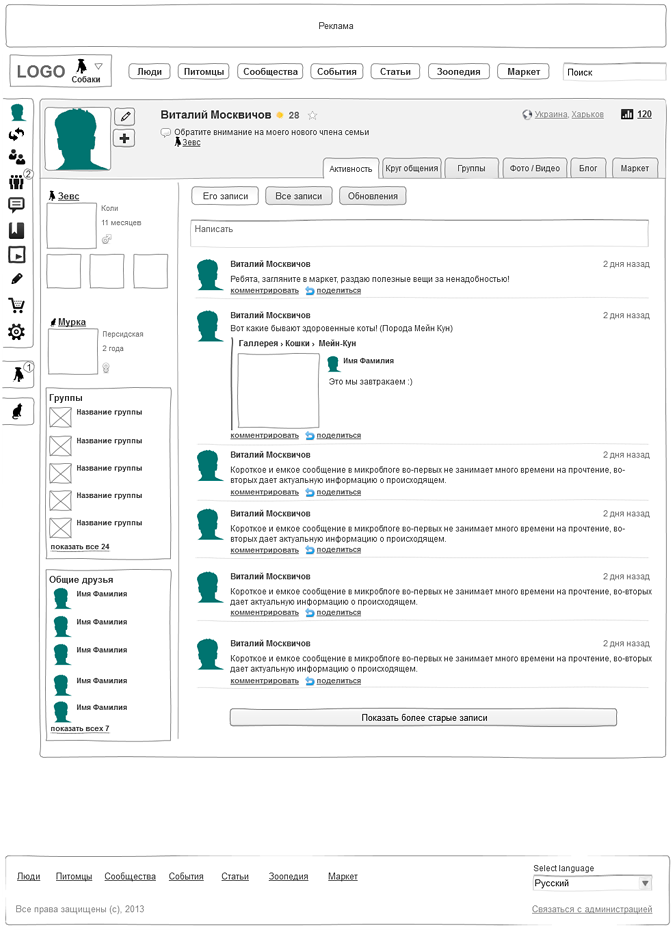
\includegraphics[scale=0.4]{images/SLJ_maket1-sm.png}
\end{figure}
\end{frame}

\begin{frame}[t]{Проектируем <<шапку>>}
\begin{enumerate}
\item Проектируем меню: 
	\begin{itemize}
		\item будет ли у нас одно меню или несколько, 
		\item будут ли там вложенности и как они будут представлены? 	
	\end{itemize}
\item проектируем шапку с элементами навигации:
	\begin{itemize}
		\item само меню, 
		\item поиск, 
		\item для магазинов - телефоны
		\item слева логотип
		\item ссылки на личный кабинет пользователя и другие персональные разделы. 
	\end{itemize}
\end{enumerate}
Шапка – самое ценное пространство, поэтому её используют для размещения самых важных элементов.
\end{frame}

\begin{frame}[t]{Примеры}
\begin{figure}[h]
\centering
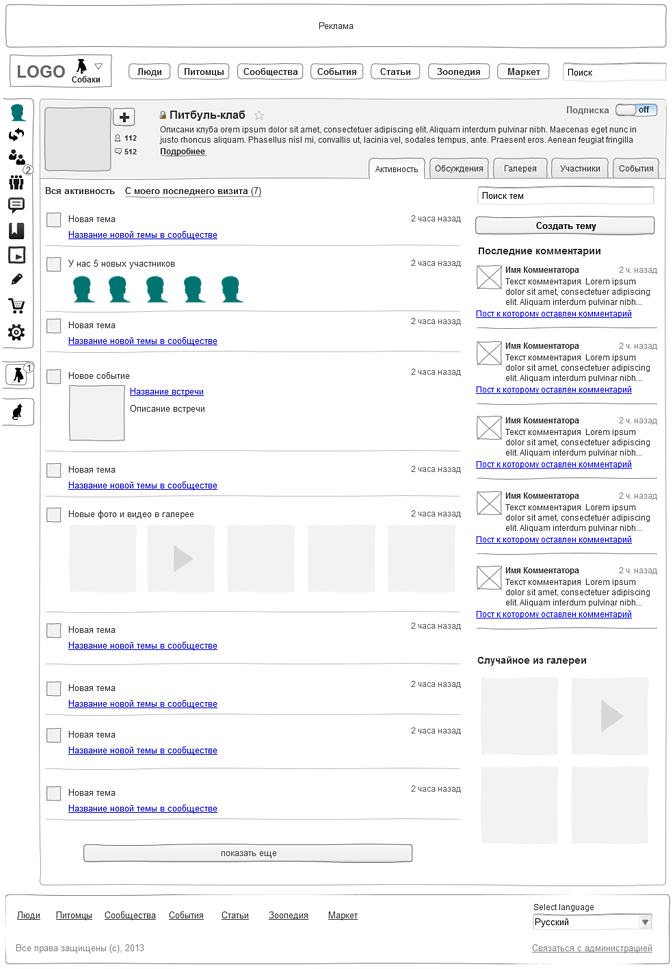
\includegraphics[scale=0.4]{images/SLJ_maket2-sm.png}
\end{figure}
\end{frame}

\begin{frame}[t]{Проектируем контентную часть}
Контентная часть будет меняться в каждом из макетов.
\begin{enumerate}
\item располагаем весь необходимый функционал и контент блоками;
\item некоторые блоки могут быть неизменными для всех страниц (так же как и шапка);
\item правая часть страницы традиционно считается «слепой зоной»: пользователи привыкли, что именно эта часть сайта посвящена рекламе и обращают мало внимание на неё, отсюда располагать там важные элементы интерфейса не рекомендуется;
\end{enumerate}
Шапка – самое ценное пространство, поэтому её используют для размещения самых важных элементов.
\end{frame}

\begin{frame}[t]{Примеры}
\begin{figure}[h]
\centering
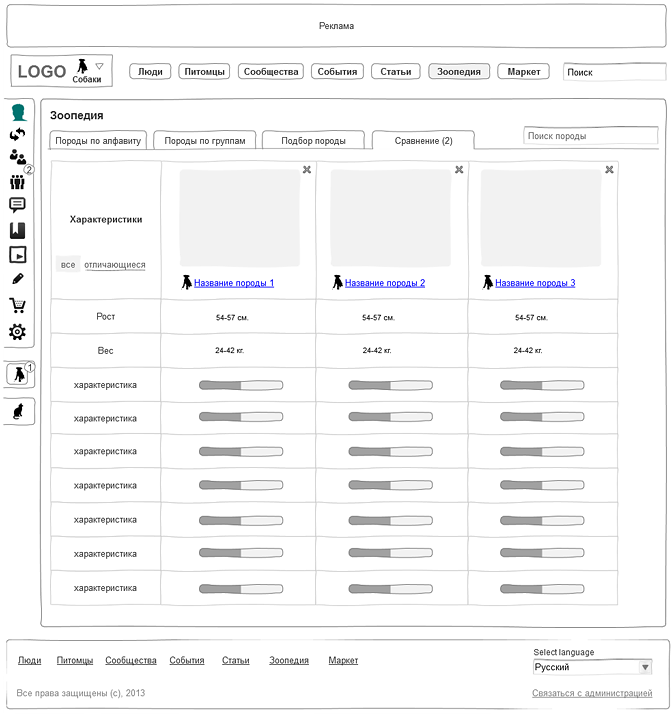
\includegraphics[scale=0.4]{images/SLJ_maket3-sm.png}
\end{figure}
\end{frame}

\begin{frame}[t]{Проектируем <<подвал>>}
Внизу страницы мы проектируем так называемый <<подвал>>, который будет неизменным для всего сайта.
\begin{enumerate}
\item обычно в подвале дублируют меню;
\item в последнее время модно делать большие подвалы, где есть:
	\begin{itemize}
	\item полная структура сайта, 
	\item информация об авторских правах,
	\item ссылки на социальные сети,
	\item ссылки на контактную информацию для связи с владельцами сайта и т.д.
	\end{itemize}
\end{enumerate}
\begin{figure}[h]
\centering
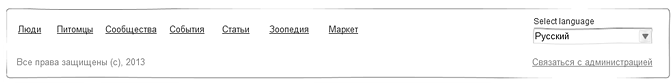
\includegraphics[scale=0.6]{images/SLJ_maket4-sm.png}
\end{figure}
\end{frame}

\begin{frame}[t]{Разное...}
\begin{enumerate}
\item учитываем в макетах \textbf{модульную сетку} - так визуально страница будет значительно легче восприниматься; 
\item нужно помнить, что пользователь смотрит слева направо и сверху вниз, это значит, что всю важную информацию нужно располагать левее и выше;
\item не забываем про брендинг: логотип должен быть заметный и обращать на себя внимание новых посетителей. Его стоит расположить в верхнем левом углу, так подсознательно он будет запоминаться пользователям;
\item изучаем наших конкурентов и смотрим, как подобный раздел реализован у них - это может натолкнуть на определенные мысли.
\item созданные прототипы мы можем тестировать с помощью наших сценариев, чтобы проверить логику еще раз, уже в интерфейсах.
\end{enumerate}
\end{frame}

\begin{frame}[t]{Что читать дальше}
\begin{itemize}
\item Fleming, Jennifer. Web Navigation: Designing the User Experience. OReilly, 1998.
\item Spolsky, Joel. User Interface Design for Programmers. Apress, 2001.
\item Tufte, Edward. Envisioning Information. Graphics Press, 1990.
\item Veen, Jeffrey. The Art and Science of Web Design. New Riders, 2000.
\end{itemize}
\end{frame}

\end{document}
